% !TeX spellcheck = pl_PL
\documentclass[a4paper,twoside]{article}
\usepackage{polski}
\usepackage[utf8]{inputenc}
\usepackage{graphicx}
\usepackage{amsmath}

\usepackage[unicode, bookmarks=true]{hyperref} %do zakładek
\usepackage{tabto} % do tabulacji
\NumTabs{6} % globalne ustawienie wielkosci tabulacji
\usepackage{array}
\usepackage{multirow}
\usepackage{array}
\usepackage{dcolumn}
\usepackage{bigstrut}
\usepackage{color}
\usepackage[usenames,dvipsnames]{xcolor}
\usepackage{svg}
\usepackage{xfrac}
\usepackage{floatrow}
\usepackage{enumitem}
\usepackage{listings,lstautogobble}
\usepackage{booktabs}
\newcommand{\tabitem}{~~\llap{\textbullet}~~}


\usepackage{multirow,tabularx}
\newcolumntype{Y}{>{\centering\arraybackslash}X}
\renewcommand{\arraystretch}{1.5}

% === Reset inkrementacji sekcji przy nowym parcie === %
\usepackage{titlesec}

\makeatletter
\@addtoreset{section}{part}
\makeatother
\titleformat{\part}[display]
{\normalfont\LARGE\bfseries\centering}{}{-60pt}{}

% === Dodanie krpki do sekcji
\titlelabel{\thetitle.\quad}


\setlength{\textheight}{24cm}
\setlength{\textwidth}{15.92cm}
\setlength{\footskip}{10mm}
\setlength{\oddsidemargin}{0mm}
\setlength{\evensidemargin}{0mm}
\setlength{\topmargin}{0mm}
\setlength{\headsep}{5mm}

\setlength{\textfloatsep}{10pt plus 1.0pt minus 2.0pt}


\begin{document}
	\bibliographystyle{plain}
	
	% !TeX spellcheck = pl_PL
% ************************************************************
% --- Strona tytułowa
% ************************************************************
\begin{titlepage}
	\begin{table}[htbp]
		\centering
		\begin{tabular}{|c|c|c|c|c|c|c|}
			\hline
			\multicolumn{7}{|c|}{\textbf{{\LARGE Grafika Komputerowa}}} \bigstrut\\[4pt]
			\hline
			Rok akademicki & Termin & Rodzaj studiów & Kierunek & Prowadzący & Grupa & Sekcja \bigstrut\\
			\hline
			\multicolumn{1}{|c|}{\multirow{2}[4]{*}{{\large 2014/2015}}} & \multicolumn{1}{c|}{{\large Piątek}} & \multicolumn{1}{c|}{\multirow{2}[4]{*}{{\large SSI}}} & \multicolumn{1}{c|}{\multirow{2}[4]{*}{{\large INF}}} & \multicolumn{1}{c|}{\multirow{2}[4]{*}{\begin{tabular}{@{}c@{}}{\large dr} \\[-9pt] {\large Ewa Lach}\end{tabular}}} & \multicolumn{1}{c|}{\multirow{2}[4]{*}{{\large GKiO3}}} & \multicolumn{1}{c|}{\multirow{2}[4]{*}{{\large 1}}} \bigstrut\\
			\cline{2-2}    \multicolumn{1}{|c|}{} & \multicolumn{1}{c|}{{\large 09:30 - 11:00}} & \multicolumn{1}{c|}{} & \multicolumn{1}{c|}{} & \multicolumn{1}{c|}{} & \multicolumn{1}{c|}{} & \multicolumn{1}{c|}{} \bigstrut\\
			\hline
		\end{tabular}%
	\end{table}%
	
	\centering
	
\includegraphics[width=0.6\textwidth]{./images/logo.png}
	\\\vspace{10mm}
	\textbf{{\huge Dokumentacja końcowa}}\\\vspace{5mm}
	\textbf{{\Huge Danmaku Shooter}}
	\\
	\vfill
	\begin{flushright}
		{\Large \textbf{Skład sekcji}:}\\
		\begin{tabular}{rr}
			{\Large Buchała} & {\Large Bartłomiej}\\[-3pt]
			{\Large Forczmański} & {\Large Mateusz}\\[-3pt]
			{\Large Motyka} & {\Large Marek}\\[-3pt]
			{\Large Wudecki} & {\Large Wojciech}
		\end{tabular}
	\end{flushright}
	
\end{titlepage}
	
	% !TeX spellcheck = pl_PL
\newpage
\part{\huge \textbf{Treść zadania}}
	
	
	% !TeX spellcheck = pl_PL
\newpage
\part{\huge \textbf{Analiza zadania}}
% --- Analiza zadania z dokumentu projektowego, poszerzoną o jasno wyszczególnione elementy, które podczas pracy zostały dodane/usunięte/uległy zmianie (z uzasadnieniem)
	\section{Sprawdzanie kolizji - okrąg czy elipsa?}
		W trakcie naszej pracy nad programem początkowo wykorzystywaliśmy okrąg do sprawdzania kolizji. Wysokość i szerokość wszystkich sprajtów była w przybliżeniu równa, więc punkty środkowe okręgu i sprajta były równe, a promieniem był krótszy z boków. Jednak po czasie pojawiły się kształty (np. bomba), dla których obsługa kolizji poprzez okrąg wyglądałaby nieatrakcyjnie. Wówczas postanowiliśmy wykorzystać elipsę. Okrąg jest jedynie specjalnym przypadkiem elipsy o równych półosiach. Gdy obiekt miał mieć hitbox w kształcie elipsy, dłuższy bok definiował długość jednej półosi, a krótszy drugiej.\\\\
		Rozwiązanie to okazało się bardzo mało efektywne - do wykrywania kolizji potrzebny były dodatkowy parametr, kąt pomiędzy obiektami. Dla jednego testu należało obliczyć ten kąt, następnie obliczyć długość promienia elipsy dla tego kąta u obu obiektów i dopiero wtedy była znane zajście kolizji. Dla hitboxów o równych osiach powodowało to mnóstwo niepotrzebnych obliczeń. Nawet pominięcie ich w przypadku równych półosi wymagało obliczania i przekazania kąta, który dla każdej elipsy był niezbędny.\\\\
		W takiej sytuacji mieliśmy dwie możliwości:
		\begin{enumerate}
			\item \textit{Zmiana elipsy wieloma okręgami} - eliminuje wykorzystanie elipsy, jednak dla każdego obiektu jest potrzebne zdefiniowanie ile okręgów potrzebuje, w którym miejscu i o jakiej wielkości, tak, by dopasować je do kształtu sprajta. Projektowanie ciała okręgów byłoby niezwykle niewygodne bez wsparcia designerskiego, którego nasza gra nie miała. 
			\item \textit{Osobne klasy dla okręgu i elipsy} - okręgu potrzebowałyby jak najmniejszej liczby danych i obliczeń, a elipsa pozostałaby obsługiwana. Wadą jest naruszenie zasad polimorfizmu - przy każdym teście okręgi nie potrzebują kąta między obiektami, więc przekazywanie ich jest zbędne i prowadzi do niepotrzebnych operacji.
		\end{enumerate}
	\section{Sprawdzanie kolizji - zastrzyk zależności}
		Rozwiązaniem problemu opisanego w powyższym rozdziale okazał się wzorzec projektowy, zastrzyk zależności (\emph{dependency injection}). Realizujemy go w ten sposób, że przy każdym teście kolizji, do jednego hitboxa wstrzykujemy drugi - pierwszy zna swoje metody działania, rzutuje drugi na odpowiedni typ i sprawdza kolizję zwracając true lub false.\\\\
		Rozwiązanie jest skuteczne, ponieważ jeżeli w teście kolizji znajduje się elipsa, to pobiera one dane jakiej jej potrzeba. Jeżeli nie, test wykonywany jest najmniejszym możliwym kosztem. Sprawdzaniem, z którym typem hitboxa mamy do czynienia zajmuje się mechanizm RTTI.
	
	% !TeX spellcheck = pl_PL
\newpage
\part{\huge \textbf{Podział pracy}}
	
	% !TeX spellcheck = pl_PL
% --- Jest to instrukcją użytkownika, z której przeciętny użytkownik powinien się dowiedzieć wszystko,
% --- co jest mu potrzebne do jego prawidłowego użytkowania. Specyfikacja zewnętrzna dotyczy
% --- interfejsu użytkownika, sposobu uruchomienia i obsługi programu, formatu danych wejściowych i wyjściowych
\newpage
\part{\huge \textbf{Specyfikacja zewnętrzna}}
	\section{Uruchomienie gry}
		Gra nie wymaga instalacji. Wystarczy otworzyć plik \textit{Danmaku.exe} i gra uruchamiania się. Po włączeniu gry pojawia się ekran powitalny wraz z menu głównym.
		\begin{center}
			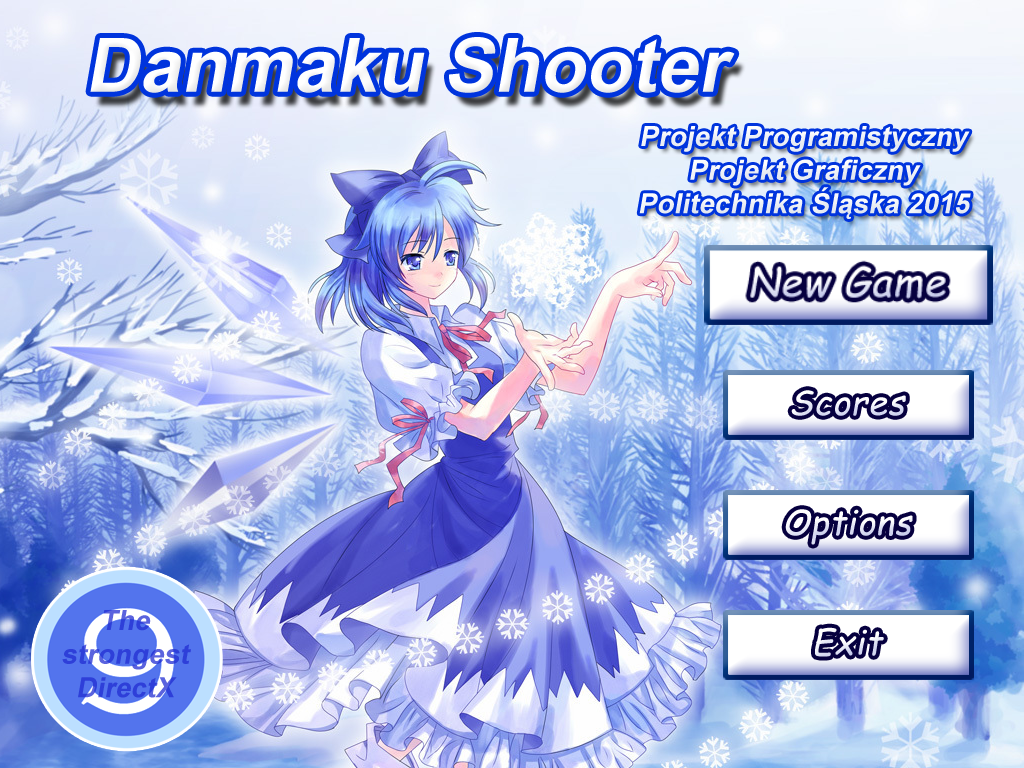
\includegraphics[width=0.7\textwidth]{./images/titlescreen_clear}
		\end{center}
		Użytkownik posiada 4 możliwości:
		\begin{itemize}
			\item Przycisk \emph{New Game} \tab - uruchomienie nowej gry
			\item Przycisk \emph{Scores} \tab - wyświetlenie wyników z poprzednich rozgrywek,
			\item Przycisk \emph{Options} \tab - konfiguracja gry
			\item Przycisk \emph{Exit} \tab - wyjście z aplikacji
		\end{itemize}
		Aktualnie wybrany przycisk pulsuje, co ułatwia wybór. Zatwierdzenia wyboru należy dokonać klikając przycisk ENTER.
	\newpage
	\section{Sterowanie}
		Domyślne sterowanie przez klawiaturę ustawione jest następująco:
		\begin{center}
			\begin{tabular}{|p{5cm}|p{5cm}|}
				\hline \textbf{Działanie} & \textbf{Klawisz(e)} \\ 
				\hline Przemieszczenie postaci & Strzałki: góra, dół, lewo, prawo \\ 
				\hline Strzelanie & Z \\
				\hline Wykorzystanie bomby & X \\
				\hline Tryb focus (spowolnienie) & Lewy Shift\\
				\hline Wyjście z gry & ESC\\
				\hline
			\end{tabular}
		\end{center}
		Klawisze sterujące można zmienić w menu \emph{Options} wedle uznania i wygody.
	\section{Konfiguracja}
		Po wybraniu przycisku \emph{Options} pojawia się menu konfiguracji.
		\begin{center}
			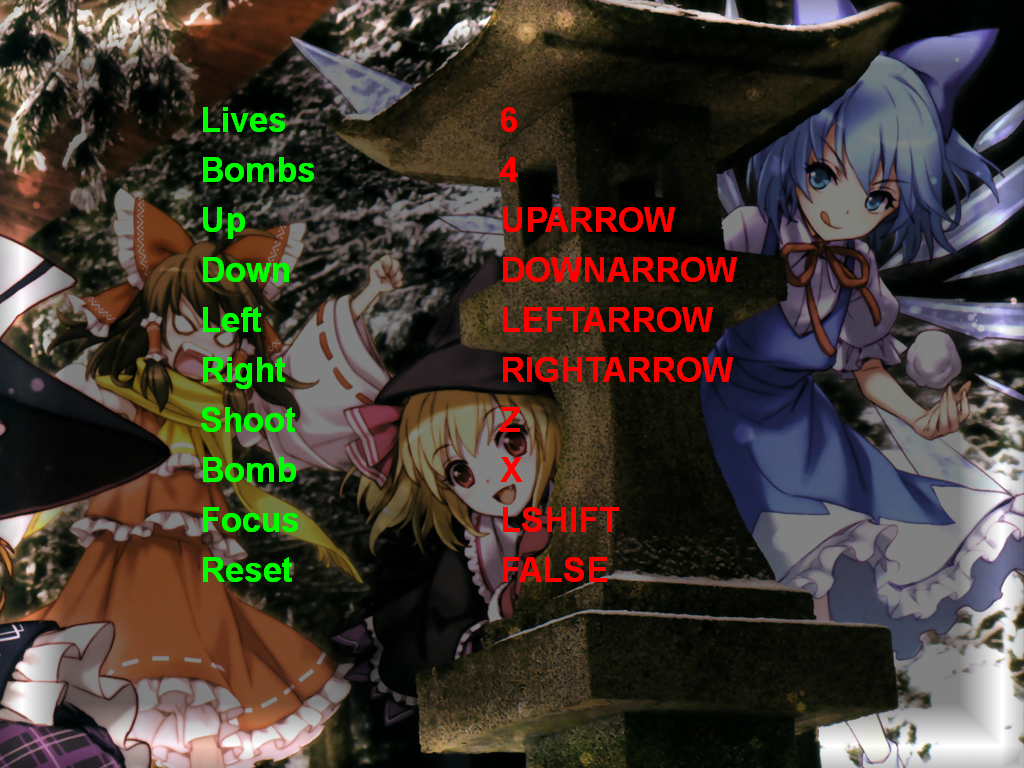
\includegraphics[width=0.7\textwidth]{./images/options_clear}
		\end{center}
		Użytkownik posiada możliwość zmiany:
		\begin{itemize}
			\item Początkowej liczby żyć, z którą rozpocznie nową grę. Aby zmienić tę wartość należy kliknąć\\ENTER, następnie strzałkami góra i dół zmienić liczbę (minimum 1, maksimum 8), i podaną wartość zatwierdzić ponownie klawiszem ENTER.
			\item Początkowej liczby bomb, z którą może rozpocząć grę. Obsługa zmiany tej liczby jest dokładnie taka sama jak dla żyć. 
			\item Klawisze sterowania. Klawiszem ENTER należy wybrać, który przycisk ma zostać zmieniony,\\a następnie potwierdzić wybór klikając wybrany przycisk na klawiaturze. Zmiana zostanie automatycznie zapisana.
			\item Przywrócenie ustawień domyślnych. Wybranie tej opcji powoduje zmianę ustawień klawiszy sterowanie na tę opisaną w podrozdziale Sterowanie, a także ustawia domyślną wartość liczby bomb\\i żyć. przywrócenie ustawień domyślnych należy zatwierdzić i można z tej decyzji się wycofać.
		\end{itemize}
		Należy pamiętać, że od startowej liczby żyć i bomb zależny jest ostateczny wynik punktowy nowej gry.
	\newpage
	\section{Tabela wyników}
		Po wybraniu przycisku \emph{Scores}, użytkownik ma możliwość podejrzenia, jakie wyniki zostały zapisane. Wyjścia z menu należy dokonać klawiszem ESC.
		\begin{center}
			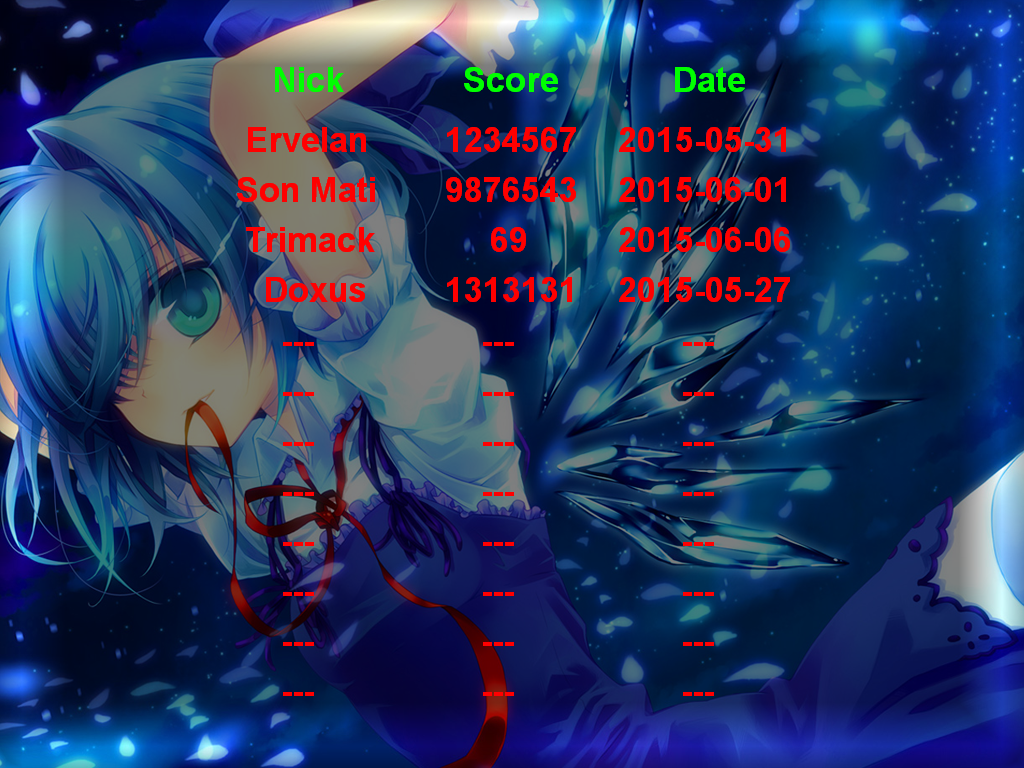
\includegraphics[width=0.7\textwidth]{./images/scores_clear}
		\end{center}
		Tabela z wynikami przedstawia rekordy z nickiem gracza, jego wynikiem punktowym oraz datą uzyskania i zapisania wyniku. Gra dopuszcza zapis tylko 12 wyników (nie muszą one być najlepszymi), w przypadku gdy gracz chce dodać swój wynik, a miejsca brakuje, musi nadpisać jeden z istniejących.
	\newpage
	\section{Gameplay}
		Po wybraniu przycisku \emph{New Game} rozpoczyna się nowa gra. Użytkownik rozpoczyna ją z zerową liczbą punktów i współczynnika \emph{graze}, oraz z najmniejszą mocą pocisków. Liczba żyć i bomb jest taka jak ustawione w Konfiguracji. Ekran gry prezentuje się następująco:
		\begin{center}
			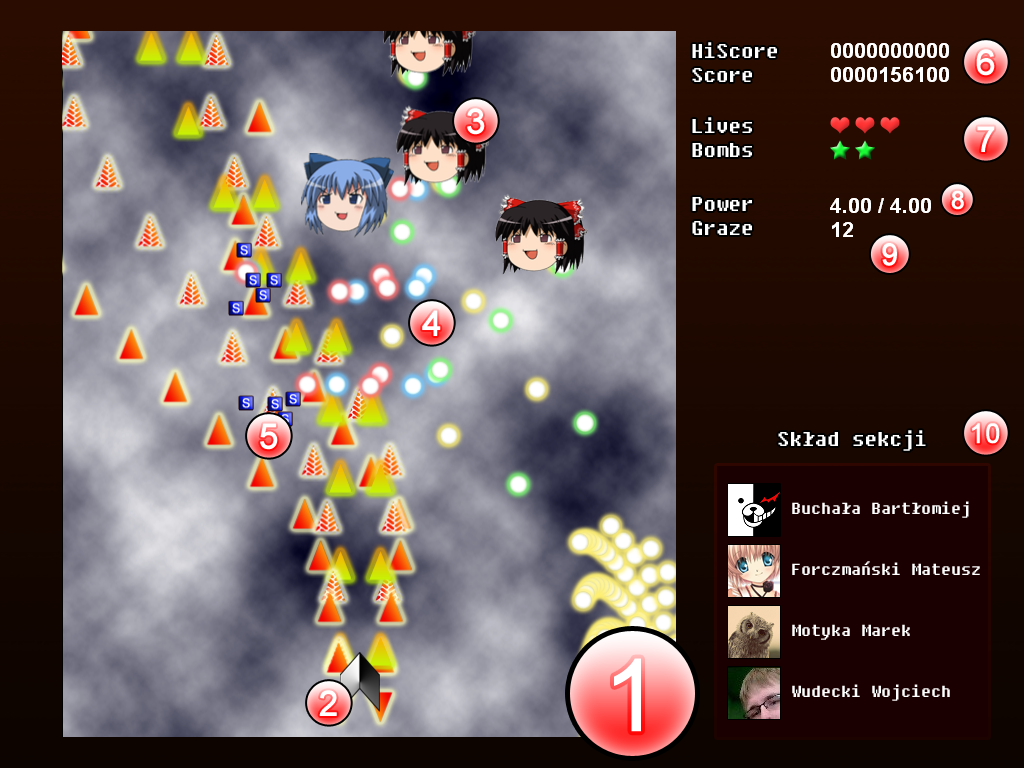
\includegraphics[width=0.7\textwidth]{./images/gameplay_clear}
		\end{center}
		\begin{enumerate}
			\item Plansza gry. Tutaj rozgrywa się cały gameplay: nie można wyjść poza jej granice, wrogowie pojawiają się zza boków i strzelają, a pociski za nimi znikają.
			\item Obiekt gracza, interaktywna część gry. Korzystając z klawiszy ruchu można nim poruszać. Jest źródłem pocisków i bomb.
			\item Wrogowie, do których należy strzelać i których należy unikać. Kontakt z nimi skutkuje stratą życia.
			\item Różnobarwne i różnokształtne wrogie pociski. Należy ich unikać, kontakt skutkuje stratą życia. Pociski mogą być wyeliminowane przez wykorzystanie bomby.
			\item Bonusy. Pojawiają się z niektórych wrogów, gdy zostaną oni pokonani. Zbieranie bonusów owocuje rożnymi efektami i wyróżniamy ich cztery rodzaje:
			\begin{itemize}
				\item Niebieski kwadrat z literą "S" \tab 
\includegraphics[width=10pt]{./images/bonusScore} \tab - dodatkowe punkty.
				\item Czerwony kwadrat z literą "P" \tab 
\includegraphics[width=10pt]{./images/bonusPower} \tab - dodatkowa moc
				\item Zielona gwiazda z literą "B" \tab 
\includegraphics[width=10pt]{./images/bonusBomb} \tab - dodatkowa bomba
				\item Czerwone serce z literą "L" \tab 
\includegraphics[width=10pt]{./images/bonusLife} \tab - dodatkowe życie
			\end{itemize}
			\item Wynik punktowy z aktualnej gry oraz porównanie go z aktualnym najlepszym wynikiem.
			\item Aktualna liczba bomb i żyć. Na początku gry jest taka, jak ustawiono w menu \emph{Options}.
			\item Aktualna moc. Można ją zwiększać zbierając odpowiedni typ bonusu. Strata życia skutkuje zmniejszeniem mocy. Zwiększanie mocy daje silniejsze pociski i zwiększa ich liczbę, co daje bardziej zaawansowany wzór.
			\item Liczba punktów \texttt{graze}. Licznik jest zwiększany, gdy gracz nie uderzy we wrogi pocisk, ale znajdzie się wystarczająco blisko, by móc powiedzieć, że się o niego "otarł". Graze zwiększa ostateczny wynik punktowy.
			\item Skład sekcji, która zrealizowała tę grę.
		\end{enumerate}
		
		
		
		
		
		
	
	% !TeX spellcheck = pl_PL
% --- W tej części należy umieścić przykład działania programu (zrzut ekranu).
\newpage
\part{\huge \textbf{Przykład działania}}
	
	% !TeX spellcheck = pl_PL
% --- Specyfikacja wewnętrzna jest dokumentacją techniczną powstałego oprogramowania.
% --- Umieścić link do automatycznie wygenerowanej dokumentacji na podstawie komentarzy.
% --- Można również opisać ciekawsze/ważniejsze elementy kodu źródłowego (funkcje, obiekty, algorytmy)
\newpage
\part{\huge \textbf{Specyfikacja wewnętrzna}}
	\section{Dokumentacja techniczna}
		Można ją znaleźć tutaj:\\\url{https://github.com/Ervie/Danmaku/blob/master/Dokumentacja/documentation.zip}
		
	\section{Wybrane funkcje}
		\subsection{Przekształcenia afiniczne}
			\begin{lstlisting}[language=C++]
				void Hitbox::Translate( D3DXVECTOR2 const & translate )
				{
					*_position += translate;
				};
			\end{lstlisting}
			\begin{lstlisting}[language=C++]
				void GameObject::Scale( float const scale )
				{
					this->scale *= scale;
					this->hitbox->Scale( scale );
				};
			\end{lstlisting}
			\begin{lstlisting}[language=C++]
				void Trajectory::GetRotation( D3DXVECTOR2 & pos, float const theta )
				{
					D3DXMATRIX mat; 
					mat._11 = cos(theta);	mat._12 = sin(theta);	mat._13 = 0.0f;		mat._14 = 0.0f;
					mat._21 = -sin(theta);	mat._22 = cos(theta);	mat._23 = 0.0f;		mat._24 = 0.0f;
					mat._31 = 0.0f;			mat._32 = 0.0f;			mat._33 = 1.0f;		mat._34 = 0.0f;
					mat._41 = 0.0f;			mat._42 = 0.0f;			mat._43 = 0.0f;		mat._44 = 1.0f;
					D3DXVec2TransformCoord(&pos, &pos, &mat);
				};
			\end{lstlisting}
	
		\subsection{Sprawdzenie kolizji gracza z pociskami}
			\begin{lstlisting}[language=C++]
				for (PatternQue::const_iterator p_it = _savedPatterns.begin(); p_it != _savedPatterns.end(); ++p_it)
				{
					std::deque<EnemyBullet*> * ep = (*p_it)->GetBullets();
					std::deque<EnemyBullet*>::const_iterator eb_it = ep->begin();
					{
						while (eb_it != ep->end())
						{
							if ((*eb_it)->GetHitbox()->TestCollision(player->GetHitbox()))
							{
								eb_it = ep->erase(eb_it);	// usunięcie pocisku z kolejki
								this->MakePlayerLoseLife();
								return;
							}
							if (eb_it != ep->end())
								eb_it++;
						}
					}
				}
			\end{lstlisting}
			\begin{lstlisting}[language=C++]
				bool HitboxCircle::TestCollision(Hitbox * collider, USHORT grazeDistance)
				{
					HitboxCircle * hCircle = dynamic_cast<HitboxCircle*>(collider);
					if (hCircle != NULL)
					{
						float distance = Vector::Length(*_position, collider->GetPosition());
						if (distance <= _radius + hCircle->GetRadius() + grazeDistance)
						{
							return true;
						}
						return false;
					}
					HitboxElipse * hElipse = dynamic_cast<HitboxElipse*>(collider);
					if (hElipse != NULL)
					{
						float distance = Vector::Length(hElipse->GetPosition(), *_position);
						float angle = Vector::Angle( *_position, hElipse->GetPosition());
						float radialLength = hElipse->GetRadialLength(angle);
						float maxDistance = _radius + radialLength + grazeDistance;
						if (distance <= maxDistance)
						{
							return true;
						}
						return false;
					}
					return false;
				};
			\end{lstlisting}
		\subsection{Obliczanie położenia na krzywej Beziera}
			\begin{lstlisting}[language=C++]
				D3DXVECTOR2 TrajectoryBezier::GetPosition( float const dis )
				{
					// znormalizowanie wartości
					float distance;
					if (_loopFlag)
						distance = fmod(dis > totalLength || dis < 0.0f ? fmod(dis + totalLength, totalLength) : dis, totalLength);
					else
						distance = dis;
					float tt = (float) distance / this->totalLength;
					// zapisanie obecnej tablicy punktów
					PointVector pointSave = PointVector(this->point);
					// Obliczenie obecnego punktu
					for (size_t k = 1; k < pointSave.size(); ++k)
					{
						for (size_t i = 0; i < pointSave.size() - k; ++i)
						{
							for	(int j = 0; j < 2; ++j)
							{
							pointSave[i][j] = (1 - tt) * pointSave[i][j] + tt * pointSave[i + 1][j];
							}
						}
					}
					return pointSave[0];
				};
			\end{lstlisting}
	
	% !TeX spellcheck = pl_PL
% -- Rozdział ten może być sprawozdaniem z procesu systematycznego testowania programu. Powinien
% -- zawierać odpowiednio przygotowane dane testowe wraz z formalnym uzasadnieniem ich doboru i
% -- ilości. W dokumentacji umieszczamy wyniki działania programu dla konkretnych danych testowych z
% -- opisem. W tym rozdziale należy umieścić wynik działania programu dla danych wejściowych. Można
% -- tu umieścić np. zrzut ekranu lub wydruk zawartości pliku wynikowego.
\newpage
\part{\huge \textbf{Testowanie i uruchamianie}}

	
	% !TeX spellcheck = pl_PL
% -- W niniejszym rozdziale można umieścić komentarze na temat pracy nad programem i inne
% -- spostrzeżenia. Można tu ustosunkować się do założeń umieszczonych w analizie zadania i stwierdzić,
% -- czy oczekiwania były trafne (np. że przewidywany algorytm okazał się odpowiedni do takiego
% -- charakteru/ takiej ilości danych lub że przyjęte rozwiązanie zbyt ograniczyło możliwości programu i
% -- że poszczególne moduły należałoby rozwijać). Rozdział ten nie wpływa na merytoryczną ocenę (o ile
% -- całe, zdefiniowane w porozumieniu z prowadzącym zadanie zostało zrealizowane).
\newpage
\part{\huge \textbf{Wnioski}}

	
\end{document}